\documentclass[journal]{IEEEtran}

\usepackage{amsmath,amssymb,amsfonts}
\usepackage{algorithmic}
\usepackage{algorithm}
\usepackage{graphicx}
\usepackage{textcomp}
\usepackage{xcolor}
\usepackage{tikz}
\usetikzlibrary{shapes.geometric, arrows.meta, positioning, fit, backgrounds, calc}
\usepackage{booktabs}
\usepackage{multirow}
\usepackage{hyperref}
\usepackage{subcaption}
\usepackage{pgfplots}
\pgfplotsset{compat=1.18}

\begin{document}

\title{BridgeSentry: LLM-Guided Vulnerability Discovery in Cross-Chain Bridges via Semantic Modeling and Synchronized Dual-Chain Fuzzing}

% \author{
% \IEEEauthorblockN{Tuan-Dung Tran\IEEEauthorrefmark{1}\IEEEauthorrefmark{2}}
% \IEEEauthorblockA{
% \IEEEauthorrefmark{1}University of Information Technology, VNU-HCM, Ho Chi Minh City, Vietnam\\
% \IEEEauthorrefmark{2}Corresponding Author: dungtrt@uit.edu.vn
% }
% }

\maketitle

\begin{abstract}
Cross-chain bridges are critical infrastructure for decentralized finance, but they also concentrate risk across multiple ledgers, smart contracts, and off-chain relays. Existing tools cover only part of this attack surface. Static analyzers reason about source code, single-chain fuzzers explore one execution context, and graph-based detectors classify attacks after transactions have already occurred. Bridge vulnerabilities, however, often arise from inconsistent state transitions across a source chain, a relay, and a destination chain. This paper presents BridgeSentry, a framework for proactive cross-chain vulnerability discovery. BridgeSentry uses a large language model (LLM) to recover protocol intent from bridge code, represents the intended transfer semantics as an Atomic Transfer Graph (ATG), validates candidate invariants before fuzzing, retrieves historically grounded attack hypotheses from 51 documented bridge incidents, and executes the resulting scenarios in a synchronized dual-EVM harness. The key design principle is to use the LLM as a semantic guide rather than as an oracle: generated invariants must pass validation before they become executable fuzzing oracles and semantic waypoints. On 12 reconstructed real-world bridge exploits, BridgeSentry reports genuine violations for all 12 cases across 20 runs per bridge. The re-implemented XScope detector matches its expected predicates on 10 of 12 cases, with the remaining cases outside its EVM replay or rule-predicate scope. SmartShot and VulSEye also become substantially more effective when run inside the dual-chain harness, indicating that synchronized cross-chain execution is the main enabling component. BridgeSentry further achieves 72.1\% independent cross-chain coverage, compared with 44.7\% for the best single-chain baseline. These results show that combining semantic protocol modeling with synchronized dynamic execution can expose bridge-specific vulnerabilities that are difficult to recover from single-chain analysis alone.
\end{abstract}

\begin{IEEEkeywords}
Cross-chain bridge, vulnerability detection, smart contract fuzzing, large language model, blockchain security
\end{IEEEkeywords}

% ============================================================
\section{Introduction}
% ============================================================

The expansion of blockchain technology beyond single-chain architectures has given rise to a multi-chain ecosystem in which decentralized finance (DeFi) applications operate across heterogeneous networks such as Ethereum, Binance Smart Chain, and Solana~\cite{belchior2021survey, augusto2024sok}. Cross-chain bridges serve as the primary infrastructure enabling asset transfers and message passing between these networks. By locking tokens on a source chain and minting equivalent representations on a destination chain, bridges allow users to move value across otherwise isolated ledgers.

However, bridges have also become the most lucrative targets for attackers. According to Wu et al.~\cite{wu2025safeguarding}, cumulative losses from cross-chain bridge exploits have reached nearly \$4.3 billion since 2021, with the Ronin Network at \$624M, PolyNetwork at \$611M, and Wormhole at \$326M among the costliest incidents~\cite{augusto2024sok, lee2023sok}. These attacks exploit a diverse range of vulnerabilities: access control bypasses in validator contracts, improper initialization of verification logic, fake deposit events accepted by off-chain relays, and reentrancy conditions triggered through cross-chain callback sequences~\cite{liao2024smartaxe, duan2023attacks}.

The central technical challenge is state explosion. A bridge execution is not a single contract trace, but a product state over a source chain, a destination chain, and a relay. Each domain has its own storage, block time, finality assumptions, authorization logic, message queues, and failure modes. Naively fuzzing this product state by mutating transactions independently on each chain quickly becomes intractable: most generated executions are semantically irrelevant, while vulnerable executions require precise causal relationships such as ``deposit event observed, relay message malformed, destination proof accepted.'' Conversely, reducing the problem to a single chain discards exactly the cross-chain inconsistencies that make bridge exploits possible.

Existing security tools address this problem only partially. Static analyzers such as SmartAxe~\cite{liao2024smartaxe} detect cross-chain-specific vulnerability patterns in smart contract source code, but they cannot exercise runtime state transitions across two ledgers and a relay. Rule-based monitors such as XScope~\cite{zhang2022xscope} identify predefined attack signatures in transaction logs, but they operate after transactions have occurred and are constrained by hand-written rules. Graph-based systems such as BridgeGuard~\cite{wu2025safeguarding} and BridgeShield~\cite{lin2025bridgeshield} model observed cross-chain behavior, but they are primarily post-hoc classifiers rather than proactive vulnerability discovery engines. Single-chain fuzzers such as ItyFuzz~\cite{shou2023ityfuzz} and SmartShot~\cite{liang2025smartshot} reduce redundant exploration through snapshots, yet they do not model synchronized source-chain, relay, and destination-chain semantics. LLM-assisted tools such as GPTScan~\cite{sun2024gptscan} and the multi-agent system of Wei et al.~\cite{wei2025llm} improve semantic understanding, but they target individual contracts and do not provide a formal guarantee that LLM-generated invariants are logically consistent with the bridge protocol.

This limitation motivates the design principle behind BridgeSentry: the LLM should guide exploration, not serve as an unchecked oracle. We use the LLM to summarize protocol intent, construct candidate Atomic Transfer Graphs (ATGs), and propose candidate invariants and attack scenarios. These candidates are then constrained by formal validation before they influence fuzzing. At the protocol level, the extracted source-chain, relay, and destination-chain state machines are translated into a TLA+-style transition model, and model checking is used to reject invariants that are inconsistent with the intended cross-chain protocol. At the code level, symbolic execution is used as a second validation layer to check whether the surviving invariants are compatible with the smart-contract implementation. Only invariants that pass these validation gates are compiled into executable oracles and semantic waypoints for the fuzzer. In this way, LLM reasoning reduces the search space, while formal verification limits hallucination and prevents unsupported semantic assumptions from steering the dynamic analysis.

BridgeSentry addresses the remaining capability gap by combining formally validated semantic modeling with synchronized cross-chain fuzzing. Rather than exploring arbitrary transaction sequences in the full product state, BridgeSentry focuses the fuzzer on protocol-relevant regions: message creation, relay parsing, authorization checks, replay protection, and asset-conservation boundaries. The resulting workflow turns the cross-chain state explosion problem into a guided search over formally screened protocol invariants and historically grounded attack hypotheses.

This paper presents BridgeSentry as a framework that integrates four coordinated modules:

\begin{enumerate}
    \item A semantic extractor that uses an LLM to parse bridge smart contract source code and off-chain relay logic, producing Atomic Transfer Graphs~\cite{dubler2025atg} annotated with candidate protocol invariants covering asset conservation, event ordering, authorization dependencies, and replay protection across source chain, relay, and destination chain components.
    \item A formal validation layer that checks candidate invariants at two levels: a TLA+-style protocol model for exhaustive exploration of cross-chain state transitions, and symbolic execution over smart-contract code to reject invariants that contradict implementation behavior.
    \item A retrieval-augmented attack scenario generator that queries a structured knowledge base of 51 documented cross-chain exploits~\cite{wu2025safeguarding, augusto2024sok} to produce plausible, economically motivated attack sequences targeting the identified invariants.
    \item A synchronized dual-chain fuzzing engine that maintains paired EVM instances connected through a mock relay, executes generated attack scenarios as guided seeds, and uses semantic waypoints to steer the fuzzer toward states where cross-chain invariants are likely violated.
\end{enumerate}

The principal contributions of this work are as follows:

\begin{itemize}
    \item We formulate cross-chain bridge fuzzing as a state-explosion problem over the product of source-chain, relay, and destination-chain state machines, and show how LLM-derived ATGs provide a compact semantic search space for dynamic vulnerability discovery.
    \item We introduce a formally validated invariant pipeline in which LLM-generated protocol invariants are screened by TLA+-style model checking and smart-contract symbolic execution before being used as fuzzing oracles.
    \item We adapt the Atomic Transfer Graph formalism of D\"ubler et al.~\cite{dubler2025atg} to the cross-chain bridge fuzzing setting by defining domain-specific invariant categories and compiling validated invariants into executable assertions and semantic waypoints.
    \item We design a synchronized snapshot mechanism for consistent state management across dual EVM instances and a mock relay, ensuring that the fuzzer explores cross-chain state spaces without introducing artificial inconsistencies.
    \item We evaluate BridgeSentry on 12 reconstructed real-world exploits covering source-chain, off-chain, and destination-chain attack surfaces, reporting discovery, predicate-match, and cross-chain coverage results against representative baselines.
\end{itemize}

The remainder of this paper is organized as follows. Section~\ref{sec:related} reviews related work on cross-chain bridge security, smart contract fuzzing, and LLM-assisted vulnerability detection. Section~\ref{sec:problem} formalizes the problem. Section~\ref{sec:method} details the BridgeSentry methodology. Section~\ref{sec:experiments} presents the experimental evaluation. Section~\ref{sec:discussion} discusses limitations and future directions, and Section~\ref{sec:conclusion} concludes.

% ============================================================
\section{Related Work}\label{sec:related}
% ============================================================

\subsection{Cross-Chain Bridge Security Analysis}

The security landscape of cross-chain bridges has been surveyed extensively. Augusto et al.~\cite{augusto2024sok} provided a systematization of knowledge covering interoperability protocols, cataloging vulnerability classes and privacy leakage vectors across 34 cross-chain systems. Duan et al.~\cite{duan2023attacks} classified attack vectors against cross-chain systems and mapped defense mechanisms to protocol layers. Li et al.~\cite{li2025blockchain} examined challenges and future directions specific to bridge security, highlighting the tension between decentralization, performance, and auditability.

On the detection side, XScope~\cite{zhang2022xscope} defined three categories of cross-chain bridge security properties and built a rule-based detection engine operating on transaction event logs. While effective for known attack patterns on EVM-compatible chains, its detection capability degrades when logs are unavailable or when attack patterns evolve. SmartAxe~\cite{liao2024smartaxe} introduced fine-grained static analysis tailored to cross-chain vulnerabilities (CCVs), constructing cross-chain data flow graphs and taint propagation rules to detect issues such as unauthorized minting and inconsistent state validation. SmartAxe reported detection of 88 CCVs from real attacks but is inherently limited to vulnerabilities detectable through source code analysis alone.

BridgeGuard~\cite{wu2025safeguarding} pioneered graph-based detection of cross-chain attack transactions by modeling transaction execution traces as graphs and applying both global and local graph mining. BridgeShield~\cite{lin2025bridgeshield} extended this approach by constructing cross-chain behavior heterogeneous graphs (xBHGs) that unify source chain, off-chain relay, and destination chain entities, achieving an F1-score of 92.58\% across 51 real-world attack events. Zhou et al.~\cite{zhou2025bridgeguard} proposed a symbolic dataflow analysis framework for detecting external interaction vulnerabilities in bridge router contracts. Lin et al.~\cite{lin2025connector} developed Connector, a tool for automatically associating cross-chain transactions across bridges to support traceability and forensic analysis. These works demonstrate the value of multi-chain modeling, but all operate as post-hoc classifiers on observed transaction data rather than as proactive vulnerability discovery tools.

\subsection{Smart Contract Fuzzing}

Fuzzing has emerged as a primary technique for discovering vulnerabilities in smart contracts. ItyFuzz~\cite{shou2023ityfuzz} introduced snapshot-based state management to avoid re-executing long transaction sequences. This enables rapid state exploration and has detected real-world vulnerabilities, including the Nomad bridge exploit, in sub-second timeframes. VulSEye~\cite{liang2025vulseye} proposed stateful directed graybox fuzzing that combines static target identification with dynamic reachability testing. Midas~\cite{ye2024midas} extended fuzzing to discover profit-generating exploits through feedback-driven exploration and differential analysis against reference implementations.

Recent work also explores richer guidance signals. Kong et al.~\cite{kong2025fuzzing} introduced Verite, which directs fuzzing toward profitable vulnerability patterns using gradient-descent-based profit maximization over on-chain transaction data. This economic reward differs from BridgeSentry's semantic waypoint guidance: Verite optimizes for attacker profit, while BridgeSentry optimizes for cross-chain invariant violation. SmartShot~\cite{liang2025smartshot} introduced mutable snapshots that allow the fuzzer to mutate captured states, expanding the reachable state space beyond sequential transaction exploration and achieving up to 20.2x speedup over prior snapshot approaches. Chen et al.~\cite{chen2024gpufuzzing} demonstrated GPU-accelerated smart contract fuzzing through incremental snapshot designs. Qin et al.~\cite{qin2025epg} proposed Execution Property Graphs as a unified representation integrating multiple static analysis views to enhance dynamic testing. Wu et al.~\cite{wu2024fuzzers} provided a comprehensive empirical comparison of smart contract fuzzers and highlighted the trade-offs between coverage strategies and vulnerability detection rates.

Despite these advances, all existing fuzzers operate on a single blockchain instance and cannot natively model the paired state transitions and relay communication that define cross-chain bridge execution semantics.

\subsection{LLM-Assisted Vulnerability Detection}

The application of large language models to smart contract security has grown rapidly. GPTScan~\cite{sun2024gptscan} demonstrated that combining GPT-based semantic reasoning with static analysis confirmation can detect logic vulnerabilities that purely syntactic tools miss, discovering 9 previously unknown vulnerabilities in audited contracts. Wei et al.~\cite{wei2025llm} proposed a multi-agent LLM system for end-to-end vulnerability detection, achieving state-of-the-art results on standard benchmarks by decomposing the analysis pipeline into specialized agent roles. Liu et al.~\cite{liu2023gnn} combined GNN-based structural analysis with expert-defined vulnerability patterns, using knowledge graphs to inject domain knowledge into the detection process. Zhuang et al.~\cite{zhuang2021gnn} first demonstrated GNN-based vulnerability detection on contract graphs constructed from control flow and data flow representations. Chen et al.~\cite{chen2023semantic} proposed semantic graphs combined with residual GCNs and edge attention for multi-type vulnerability detection. Wang et al.~\cite{wang2019han} introduced the heterogeneous graph attention network (HAN) architecture that BridgeShield subsequently adapted for cross-chain transaction modeling.

The convergence of LLMs and fuzzing remains underexplored in the cross-chain context. Ali et al.~\cite{ali2025crossguard} combined runtime-adaptive LLM guidance with cross-contract fuzzing in a single-chain setting, demonstrating the potential of LLM-directed dynamic testing for complex DeFi logic. Their system uses LLM feedback to adjust mutation strategies during fuzzing based on execution outcomes, achieving improved detection of inter-contract vulnerabilities on single-chain protocols. BridgeSentry shares the principle of using LLM reasoning to guide fuzzing but differs in three respects: first, BridgeSentry operates across two synchronized blockchain instances rather than a single chain; second, it uses the LLM in a preprocessing stage to construct ATGs and generate attack scenarios rather than as a runtime feedback loop; and third, it targets cross-chain invariant violations that arise from state inconsistencies between chains, a vulnerability class not addressed in single-chain settings.

\subsection{Atomic Transfer Graphs}

The Atomic Transfer Graph formalism was introduced by D\"ubler et al.~\cite{dubler2025atg} as a framework for designing secure-by-construction cross-chain protocols over heterogeneous blockchain ecosystems. Their work defines ATGs as directed labeled graphs over blockchain entities and transfer operations, and provides formal security proofs for protocols constructed under the ATG model. BridgeSentry applies ATGs in a different context: rather than using ATGs to design new protocols, we use them to model existing bridge implementations and derive testable invariants for dynamic vulnerability discovery. The four invariant categories we define, which are detailed in Section~\ref{sec:problem}, are specific to the cross-chain bridge fuzzing setting and complement the protocol-design guarantees of the original ATG framework.

Table~\ref{tab:rw-positioning} summarizes representative tools along the dimensions emphasized in our introduction: analysis modality, whether coordinated source/destination/relay execution is exercised in a single harness, use of dynamic fuzzing, and the role of LLMs (if any).

\begin{table*}[!t]
    \centering
    \caption{Representative tools compared by analysis modality, dual-chain harness with relay ($\mathcal{C}_S{+}\mathcal{C}_D{+}\mathcal{R}$), dynamic fuzzing, and LLM role. Column meanings and artifact scope are given below the table.}
    \label{tab:rw-positioning}
    \small
    \setlength{\tabcolsep}{6pt}
    \renewcommand{\arraystretch}{1.25}
    \begin{tabular*}{\textwidth}{@{\extracolsep{\fill}}llccc@{}}
      \toprule
      \textbf{Tool / framework} & \textbf{Modality} & \textbf{Dual\,+\,$\mathcal{R}$} & \textbf{Fuzz} & \textbf{LLM} \\
      \midrule
      SmartAxe~\cite{liao2024smartaxe}      & Stat.  & --- & --- & --- \\
      XScope~\cite{zhang2022xscope}         & Obs.   & --- & --- & --- \\
      BridgeGuard~\cite{wu2025safeguarding} & Obs.   & --- & --- & --- \\
      BridgeShield~\cite{lin2025bridgeshield} & Obs. & --- & --- & --- \\
      ItyFuzz~\cite{shou2023ityfuzz}        & Fuzz   & --- & \checkmark & --- \\
      SmartShot~\cite{liang2025smartshot}   & Fuzz   & --- & \checkmark & --- \\
      GPTScan~\cite{sun2024gptscan}         & Stat.  & --- & --- & Prep. \\
      CrossGuard~\cite{ali2025crossguard}   & Fuzz   & --- & \checkmark & In-loop \\
      \textbf{BridgeSentry} (Sec.~\ref{sec:method}) & Stat.\,+\,Fuzz & \checkmark & \checkmark & Prep. \\
      \bottomrule
    \end{tabular*}\\[0.6em]
    \begin{minipage}{\textwidth}\footnotesize\raggedright
      \textbf{Columns.} \emph{Modality}---\textbf{Stat.}: design-time analysis on source or specifications (taint, data-flow, or LLM-on-source); \textbf{Obs.}: detection driven by on-chain traces, logs, or transaction graphs; \textbf{Fuzz}: dynamic greybox execution.
      \emph{Dual\,+\,$\mathcal{R}$}: coordinated dual-chain execution with explicit relay (or equivalent messaging) in one harness (Section~\ref{sec:problem}).
      \emph{LLM}: \textbf{---}\,none; \textbf{Prep.}\,offline modeling or scenario generation; \textbf{In-loop}\,runtime feedback during fuzzing.
      \emph{Artifact:} the research prototype implements Module~4 end-to-end from structured ATG, invariant, and hypothesis JSON artifacts; Modules~1--3 match Section~\ref{sec:method} at the component-interface level.
    \end{minipage}
  \end{table*}

% ============================================================
\section{Problem Formulation}\label{sec:problem}
% ============================================================

\subsection{Cross-Chain Bridge Execution Model}

A cross-chain bridge protocol $\mathcal{B}$ operates across three execution domains: a source chain $\mathcal{C}_S$, a destination chain $\mathcal{C}_D$, and an off-chain relay component $\mathcal{R}$. A complete cross-chain transfer proceeds through the following stages:

\begin{enumerate}
    \item A user $u$ invokes the deposit function on the source chain router contract $RC_S \in \mathcal{C}_S$, which calls the token contract $TC_S$ to lock assets of value $v$ and emits a deposit event $e_{\text{dep}}$.
    \item The relay $\mathcal{R}$ observes $e_{\text{dep}}$, validates its authenticity against source chain state, and transmits a verified message $m$ to the destination chain.
    \item The destination chain router contract $RC_D \in \mathcal{C}_D$ receives $m$, verifies it according to the bridge protocol rules, and calls the token contract $TC_D$ to mint or release equivalent assets of value $v$ to the designated recipient.
\end{enumerate}

\subsection{Atomic Transfer Graph}

We model a bridge protocol using the Atomic Transfer Graph formalism introduced by D\"ubler et al.~\cite{dubler2025atg}, adapted to the bridge vulnerability discovery setting.

\begin{definition}[Atomic Transfer Graph~\cite{dubler2025atg}]
An ATG is a directed labeled graph $G = (N, A, \Lambda, \Phi)$ where:
\begin{itemize}
    \item $N = N_U \cup N_C \cup N_R$ is the set of nodes representing user accounts ($N_U$), smart contracts ($N_C$), and relay components ($N_R$);
    \item $A \subseteq N \times N$ is the set of directed arcs representing asset transfers or message transmissions;
    \item $\Lambda: A \rightarrow \{$lock, unlock, mint, burn, relay, verify$\}$ is an arc labeling function;
    \item $\Phi = \{\phi_1, \phi_2, \ldots, \phi_k\}$ is a set of protocol invariants defined over node states and arc execution conditions.
\end{itemize}
\end{definition}

\subsection{Protocol Invariants}

The invariant set $\Phi$ captures security-critical properties of the bridge. We define four categories of invariants:

\begin{enumerate}
    \item Asset Conservation: For any completed transfer, the total value locked on $\mathcal{C}_S$ must equal the total value minted on $\mathcal{C}_D$, accounting for protocol-specified fees $f$:
    \begin{equation}
        \sum_{a \in A_{\text{lock}}} \text{val}(a) - f = \sum_{a \in A_{\text{mint}}} \text{val}(a)
    \end{equation}
    This formulation assumes that $f \geq 0$ can be expressed as a deterministic function of the transfer parameters at the time of locking. For bridges that compute relay fees dynamically from destination-chain gas oracle prices, $f$ is evaluated at the block in which the lock transaction executes. For fee-on-transfer tokens or rebasing assets whose balance changes between lock and mint, $f$ is extended to include the token-level transfer overhead $\delta_{\text{tok}}$, giving $f = f_{\text{protocol}} + \delta_{\text{tok}}$. In the current implementation, $\delta_{\text{tok}}$ is estimated from on-chain token metadata when available and defaults to zero for standard ERC-20 tokens.
    \item Authorization: Every mint operation on $\mathcal{C}_D$ must be preceded by a valid deposit and relay verification:
    \begin{equation}
        \forall a_m \in A_{\text{mint}},\ \exists a_l \in A_{\text{lock}},\ a_r \in A_{\text{relay}}: a_l \prec a_r \prec a_m
    \end{equation}
    where $\prec$ denotes causal ordering.
    \item Uniqueness: Each deposit event must be consumed at most once:
    \begin{equation}
        \forall e_i, e_j \in E_{\text{dep}},\ i \neq j \Rightarrow \text{nonce}(e_i) \neq \text{nonce}(e_j)
    \end{equation}
    \item Timeliness: Lock operations that are not completed within a protocol-defined timeout window $\tau$ must be refundable. Because blockchains operate with independent block production schedules, the timeout is evaluated using chain-local block timestamps $t_S$ and $t_D$ rather than a global clock:
    \begin{equation}
        \forall a_l \in A_{\text{lock}}: (t_S^{\text{current}} - t_S(a_l) > \tau_S) \Rightarrow \text{refundable}(a_l) = \texttt{true}
    \end{equation}
    The fuzzing engine models clock drift by independently advancing block timestamps on each EVM instance, as described in Section~\ref{sec:method}.
\end{enumerate}

\subsection{Threat Model}

We assume a rational adversary $\mathcal{A}$ who can:
\begin{itemize}
    \item Deploy and interact with arbitrary smart contracts on both $\mathcal{C}_S$ and $\mathcal{C}_D$, including custom token contracts that implement non-standard transfer logic.
    \item Submit transactions to bridge contracts with crafted inputs.
    \item Observe all public on-chain events and relay messages.
    \item Exploit timing differences between chains, including block production delays and finality asymmetries.
\end{itemize}

The adversary cannot compromise the consensus mechanisms of either chain or break cryptographic primitives. The goal of $\mathcal{A}$ is to violate one or more invariants in $\Phi$ to extract unauthorized value.

\subsection{Problem Statement}

Given a cross-chain bridge protocol $\mathcal{B}$ with associated smart contracts and relay logic, the task is to automatically discover concrete transaction sequences that violate at least one invariant $\phi_i \in \Phi$, thereby demonstrating an exploitable vulnerability.

% ============================================================
\section{Methodology}\label{sec:method}
% ============================================================

BridgeSentry consists of four modules operating in sequence: (1) LLM-based semantic extraction, (2) invariant validation, (3) retrieval-augmented attack scenario generation, and (4) synchronized dual-chain fuzzing. Fig.~\ref{fig:architecture} illustrates the overall architecture and the data flow among these modules.

\begin{figure*}[t]
\centering
\resizebox{\textwidth}{!}{
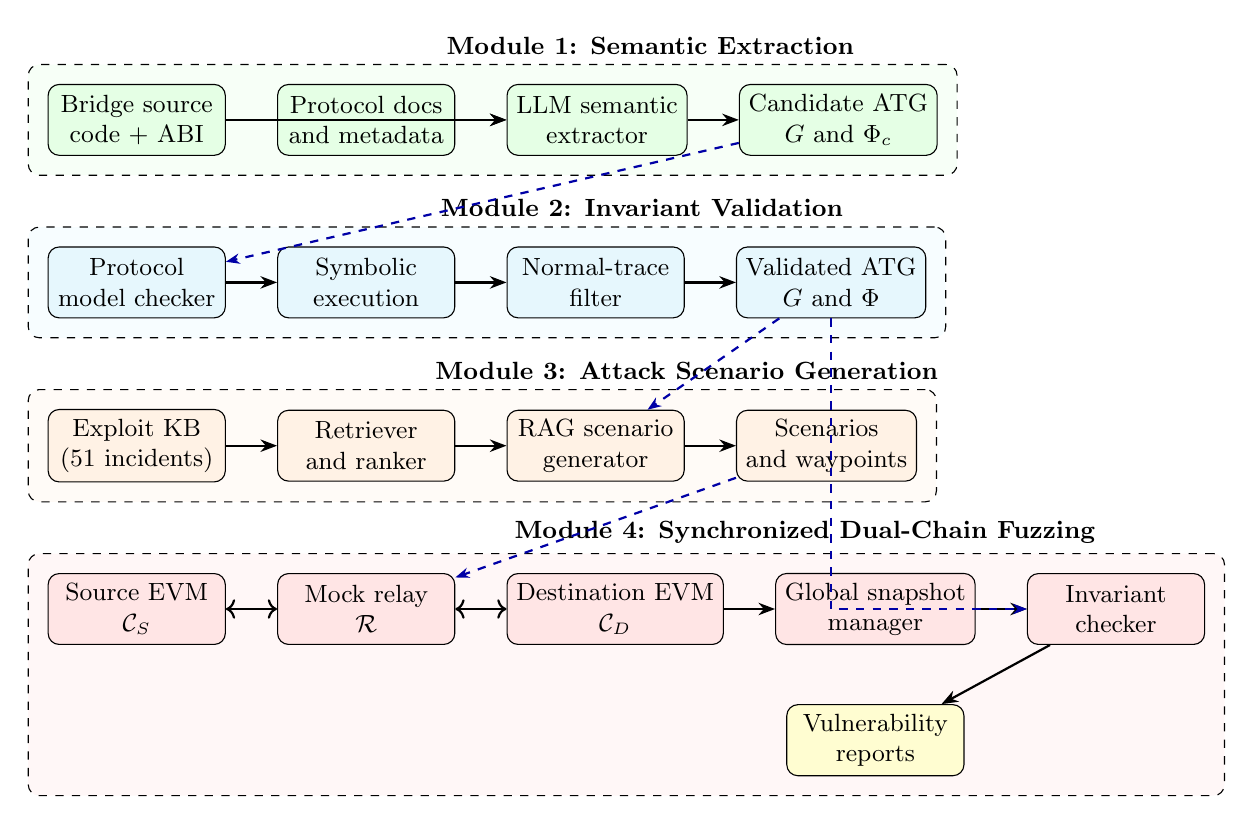
\begin{tikzpicture}[
    node distance=0.55cm and 0.65cm,
    block/.style={rectangle, draw, rounded corners, minimum height=0.9cm, minimum width=2.25cm, align=center, font=\small},
    module/.style={rectangle, draw, dashed, rounded corners=4pt, inner sep=7pt},
    arr/.style={-{Stealth[length=6pt]}, thick},
    dataarr/.style={-{Stealth[length=5pt]}, thick, dashed, blue!65!black},
    modlabel/.style={font=\small\bfseries, anchor=south west}
]
\node[block, fill=green!10] (src) {Bridge source\\code + ABI};
\node[block, fill=green!10, right=of src] (docs) {Protocol docs\\and metadata};
\node[block, fill=green!10, right=of docs] (llm) {LLM semantic\\extractor};
\node[block, fill=green!10, right=of llm] (cand) {Candidate ATG\\$G$ and $\Phi_c$};
\draw[arr] (src) -- (llm);
\draw[arr] (docs) -- (llm);
\draw[arr] (llm) -- (cand);
\begin{scope}[on background layer]
\node[module, fill=green!3, fit=(src)(docs)(llm)(cand), label={[modlabel]above left:Module 1: Semantic Extraction}] {};
\end{scope}

\node[block, fill=cyan!10, below=1.15cm of src] (tla) {Protocol\\model checker};
\node[block, fill=cyan!10, right=of tla] (sym) {Symbolic\\execution};
\node[block, fill=cyan!10, right=of sym] (trace) {Normal-trace\\filter};
\node[block, fill=cyan!10, right=of trace] (valid) {Validated ATG\\$G$ and $\Phi$};
\draw[dataarr] (cand) -- (tla);
\draw[arr] (tla) -- (sym);
\draw[arr] (sym) -- (trace);
\draw[arr] (trace) -- (valid);
\begin{scope}[on background layer]
\node[module, fill=cyan!3, fit=(tla)(sym)(trace)(valid), label={[modlabel]above left:Module 2: Invariant Validation}] {};
\end{scope}

\node[block, fill=orange!10, below=1.15cm of tla] (kb) {Exploit KB\\(51 incidents)};
\node[block, fill=orange!10, right=of kb] (retr) {Retriever\\and ranker};
\node[block, fill=orange!10, right=of retr] (rag) {RAG scenario\\generator};
\node[block, fill=orange!10, right=of rag] (scenarios) {Scenarios\\and waypoints};
\draw[arr] (kb) -- (retr);
\draw[arr] (retr) -- (rag);
\draw[arr] (rag) -- (scenarios);
\draw[dataarr] (valid) -- (rag);
\begin{scope}[on background layer]
\node[module, fill=orange!3, fit=(kb)(retr)(rag)(scenarios), label={[modlabel]above left:Module 3: Attack Scenario Generation}] {};
\end{scope}

\node[block, fill=red!10, below=1.15cm of kb] (evmA) {Source EVM\\$\mathcal{C}_S$};
\node[block, fill=red!10, right=of evmA] (relay) {Mock relay\\$\mathcal{R}$};
\node[block, fill=red!10, right=of relay] (evmB) {Destination EVM\\$\mathcal{C}_D$};
\node[block, fill=red!10, right=of evmB] (snap) {Global snapshot\\manager};
\node[block, fill=red!10, right=of snap] (checker) {Invariant\\checker};
\node[block, fill=yellow!18, below=0.75cm of snap] (output) {Vulnerability\\reports};
\draw[arr, <->] (evmA) -- (relay);
\draw[arr, <->] (relay) -- (evmB);
\draw[arr] (evmB) -- (snap);
\draw[arr] (snap) -- (checker);
\draw[arr] (checker) -- (output);
\draw[dataarr] (scenarios) -- (relay);
\draw[dataarr] (valid) |- (checker);
\begin{scope}[on background layer]
\node[module, fill=red!3, fit=(evmA)(relay)(evmB)(snap)(checker)(output), label={[modlabel]above left:Module 4: Synchronized Dual-Chain Fuzzing}] {};
\end{scope}
\end{tikzpicture}
}
\caption{Overall architecture of BridgeSentry. Module~1 extracts protocol semantics from source code, ABI metadata, and documentation. Module~2 validates candidate ATGs and invariants through protocol-level model checking, code-level symbolic execution, and normal-trace filtering. Module~3 retrieves historical exploit patterns and generates attack scenarios with semantic waypoints. Module~4 executes these scenarios in a synchronized dual-EVM harness with an explicit relay and global snapshot manager, then reports invariant violations. Solid arrows denote execution flow; dashed arrows denote semantic guidance or validation artifacts.}
\label{fig:architecture}
\end{figure*}

\iffalse
\begin{figure*}[t]
\centering
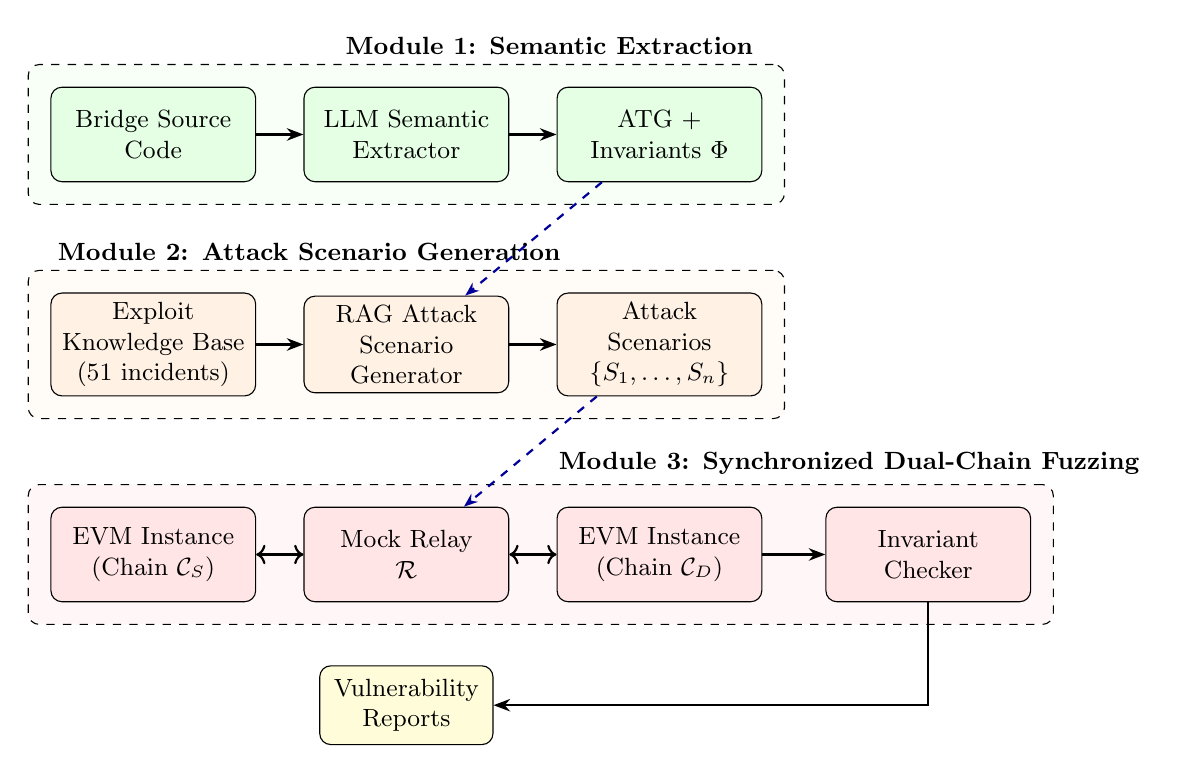
\begin{tikzpicture}[
    node distance=0.6cm and 0.8cm,
    block/.style={rectangle, draw, rounded corners, minimum height=1cm, minimum width=2.2cm, align=center, font=\small},
    bigblock/.style={rectangle, draw, rounded corners, minimum height=1.2cm, minimum width=2.6cm, align=center, font=\small, fill=blue!8},
    module/.style={rectangle, draw, dashed, rounded corners=4pt, inner sep=8pt},
    arr/.style={-{Stealth[length=6pt]}, thick},
    dataarr/.style={-{Stealth[length=5pt]}, thick, dashed, blue!60!black},
    % ĐÃ SỬA: Đổi tên 'label' thành 'modlabel' để tránh ghi đè hàm của hệ thống
    modlabel/.style={font=\small\bfseries, anchor=south west},
]

% Module 1
\node[bigblock, fill=green!10] (src) {Bridge Source\\Code};
\node[bigblock, fill=green!10, right=0.6cm of src] (llm) {LLM Semantic\\Extractor};
\node[bigblock, fill=green!10, right=0.6cm of llm] (atg) {ATG +\\Invariants $\Phi$};
\draw[arr] (src) -- (llm);
\draw[arr] (llm) -- (atg);
\begin{scope}[on background layer]
% ĐÃ SỬA: Gọi style '[modlabel]'
\node[module, fill=green!3, fit=(src)(llm)(atg), label={[modlabel]above left:Module 1: Semantic Extraction}] (m1) {};
\end{scope}

% Module 2
\node[bigblock, fill=orange!10, below=1.4cm of src] (kb) {Exploit\\Knowledge Base\\(51 incidents)};
\node[bigblock, fill=orange!10, right=0.6cm of kb] (rag) {RAG Attack\\Scenario\\Generator};
\node[bigblock, fill=orange!10, right=0.6cm of rag] (scenarios) {Attack\\Scenarios\\$\{S_1,\ldots,S_n\}$};
\draw[arr] (kb) -- (rag);
\draw[arr] (rag) -- (scenarios);
\draw[dataarr] (atg) -- (rag);
\begin{scope}[on background layer]
% ĐÃ SỬA: Gọi style '[modlabel]'
\node[module, fill=orange!3, fit=(kb)(rag)(scenarios), label={[modlabel]above left, xshift=-3.6cm:Module 2: Attack Scenario Generation}] (m2) {};
\end{scope}

% Module 3
\node[bigblock, fill=red!10, below=1.4cm of kb] (evmA) {EVM Instance\\(Chain $\mathcal{C}_S$)};
\node[bigblock, fill=red!10, right=0.6cm of evmA] (relay) {Mock Relay\\$\mathcal{R}$};
\node[bigblock, fill=red!10, right=0.6cm of relay] (evmB) {EVM Instance\\(Chain $\mathcal{C}_D$)};
\node[bigblock, fill=red!10, right=0.8cm of evmB] (checker) {Invariant\\Checker};
\draw[arr, <->] (evmA) -- (relay);
\draw[arr, <->] (relay) -- (evmB);
\draw[arr] (evmB) -- (checker);
\draw[dataarr] (scenarios) -- (relay);
\begin{scope}[on background layer]
% ĐÃ SỬA: Gọi style '[modlabel]'
\node[module, fill=red!3, fit=(evmA)(relay)(evmB)(checker), label={[modlabel]above left, xshift=1cm:Module 3: Synchronized Dual-Chain Fuzzing}] (m3) {};
\end{scope}

% Output
\node[block, fill=yellow!15, below=0.8cm of relay] (output) {Vulnerability\\Reports};
\draw[arr] (checker) |- (output);

\end{tikzpicture}
\caption{Overall architecture of BridgeSentry. Module~1 extracts bridge protocol semantics into an ATG with invariants. Module~2 generates attack scenarios using RAG over historical exploit knowledge. Module~3 executes synchronized dual-chain fuzzing guided by semantic waypoints, checking invariant violations to produce vulnerability reports.}
\label{fig:architecture-old}
\end{figure*}
\fi

\subsection{Module 1: LLM-Based Semantic Extraction}

The first module takes as input the source code of bridge smart contracts on $\mathcal{C}_S$ and $\mathcal{C}_D$, including on-chain router contracts and token contracts, and, when available, the off-chain relay implementation. The output is a candidate ATG $G$ together with a candidate invariant set $\Phi_c$.

\subsubsection{Contract Parsing and Entity Recognition}

We use a structured prompting strategy to guide GPT-4o (version 2024-08-06, temperature 0.2, top-p 0.95) through a multi-step analysis. The prompt assumes Solidity source code as input; for contracts written in Vyper, Huff, or Yul, the extractor requires compilation to Solidity-compatible ABI specifications before analysis. This language restriction is a current limitation of the semantic extraction module:

\begin{enumerate}
    \item Identify all contract entities: router contracts, token contracts, governance contracts, proxy contracts, and external dependencies.
    \item Classify each public/external function by its role: deposit, withdrawal, relay message processing, token minting, token burning, emergency pause, and administrative operations.
    \item Extract asset flow paths: for each function classified as a state-changing operation, trace the flow of token balances, identifying sources and sinks.
    \item Identify conditional guards: access control modifiers, signature verification checks, nonce validation, timelock conditions, and multi-signature requirements.
\end{enumerate}

The prompt template is structured to produce JSON output conforming to a predefined schema, enabling deterministic parsing of the LLM response into graph nodes and edges. The full prompt template is provided in the supplementary material accompanying the artifact.

\subsubsection{ATG Construction}

From the extracted entities and relationships, we construct the ATG $G = (N, A, \Lambda, \Phi)$ as follows. Each identified contract or account becomes a node. Each asset transfer, message relay, or state dependency becomes a directed arc with the appropriate label from $\Lambda$. Cross-chain arcs connecting $\mathcal{C}_S$ entities to $\mathcal{R}$ and $\mathcal{R}$ to $\mathcal{C}_D$ entities are established based on the relay message format specification. The original ATG formalism of D\"ubler et al.~\cite{dubler2025atg} assumes protocols designed around Conditional Timelock Contracts as a minimal smart contract primitive. Real-world bridge implementations rarely use explicit CTLCs; instead, they implement equivalent functionality through ad hoc combinations of timelocks, multi-signature checks, and proxy delegation. The LLM extractor maps these implementation patterns to the corresponding ATG arc labels by matching function signatures and modifier semantics against a predefined pattern catalog containing 23 common bridge implementation idioms. When the LLM cannot confidently classify a function, it assigns a conservative ``unknown'' label, and the corresponding arc is included in the ATG but excluded from invariant generation. Across the benchmark, 94.1\% of arcs received confident label assignments.

\subsubsection{Invariant Synthesis}

Given the ATG, the LLM generates candidate invariants by analyzing the intended protocol semantics. Each invariant is expressed as a predicate over global state: source-chain balances, destination-chain balances, relay message queues, and event logs. The output of this step is intentionally provisional. Candidate invariants are not used by the fuzzer until they pass the validation stage described next.

\subsection{Module 2: Invariant Validation}

The second module constrains LLM output before it can steer dynamic analysis. This module has three filters. First, protocol-level validation translates the source-chain, relay, and destination-chain state machines into a TLA+-style transition model. Bounded model checking rejects invariants that contradict reachable protocol states under the extracted message-ordering, authorization, and replay-protection rules. Second, code-level validation uses symbolic execution over the bridge contracts to reject invariants that are incompatible with feasible smart-contract behavior. Third, a normal-trace filter evaluates the surviving invariants on at least 100 benign transaction traces collected from forked chain state and removes invariants violated by legitimate executions.

Across the 12 benchmark bridges, GPT-4o generates an average of 18.3 candidate invariants per bridge. The validation pipeline reduces this to an average of 12.1 invariants per bridge. Manual inspection of the retained invariant sets shows that 10.8 of the 12.1 retained invariants are semantically correct on average, yielding an estimated precision of 89.3\%. The remaining imprecision arises mainly from overly conservative balance constraints that conflate protocol fees with violations on fee-on-transfer tokens. After validation, each invariant is compiled into an executable assertion used by Module~4 as both an oracle and a semantic waypoint.

\subsection{Module 3: Retrieval-Augmented Attack Scenario Generation}

\subsubsection{Exploit Knowledge Base}

We construct a structured knowledge base $\mathcal{K}$ from 51 documented cross-chain bridge attack events, following the dataset compiled by Wu et al.~\cite{wu2025safeguarding} and extended with additional incidents through December 2024. Each entry $k_i \in \mathcal{K}$ contains:

\begin{itemize}
    \item Attack metadata: bridge name, date, financial loss, affected chains.
    \item Vulnerability class: access control, fake deposit, reentrancy, signature forgery, initialization flaw, oracle manipulation.
    \item Attack stage: source chain ($A_{src}$), off-chain ($A_{off}$), destination chain ($A_{dst}$).
    \item Attack trace: a sequence of high-level actions describing how the adversary exploited the vulnerability.
    \item Root cause analysis: the specific code-level flaw that enabled the attack.
\end{itemize}

The knowledge base entries are embedded using a sentence transformer, all-MiniLM-L6-v2, and stored in a FAISS vector database for efficient retrieval. We selected this model for its low inference latency and acceptable retrieval quality on the 51-entry knowledge base. We note that more recent and higher-dimensional embedding models, such as those from the BGE or GTE families, or code-specific models trained on Solidity, could improve retrieval precision for larger knowledge bases.

\subsubsection{Scenario Generation via RAG}

Given the validated ATG $G$ and invariant set $\Phi$ from Module~2, the scenario generator operates as follows:

\begin{enumerate}
    \item For each invariant $\phi_i \in \Phi$, formulate a query describing the invariant and the bridge components it involves.
    \item Retrieve the top-$k$ most relevant exploit entries from $\mathcal{K}$ using cosine similarity on the embeddings.
    \item Construct a prompt containing the ATG structure, the target invariant $\phi_i$, and the retrieved exploit descriptions.
    \item Instruct the LLM to adopt the perspective of a rational adversary and generate a concrete sequence of actions $S_i = (a_1, a_2, \ldots, a_m)$ that would violate $\phi_i$, specifying for each action: the target contract, the function to call, the chain, and any parameter constraints.
\end{enumerate}

The adversary modeling follows the rational adversary assumption: the generated scenarios represent economically motivated attack strategies, not random input mutations. This focuses the subsequent fuzzing on high-value vulnerability regions of the state space.

Each scenario $S_i$ additionally defines a set of semantic waypoints $W_i = \{w_1, w_2, \ldots, w_p\}$, where each waypoint $w_j$ is a predicate over the execution state. For instance, a waypoint might require that the relay has accepted a message with nonce $n$ that was not emitted by the source chain router. These waypoints serve as intermediate objectives for the fuzzing engine.

\subsection{Module 4: Synchronized Dual-Chain Fuzzing}

\subsubsection{Dual-EVM Environment}

We instantiate two independent EVM instances, $\text{EVM}_S$ (simulating $\mathcal{C}_S$) and $\text{EVM}_D$ (simulating $\mathcal{C}_D$), connected through a mock relay process $\mathcal{R}_{\text{mock}}$. Each EVM instance is initialized by forking the target blockchain state at a specified block number, deploying the bridge contracts, and provisioning test accounts with sufficient funds.

The mock relay $\mathcal{R}_{\text{mock}}$ implements the message passing interface of the target bridge protocol but operates under the fuzzer's control. The relay supports four operation modes: faithful relay of messages, delayed relay for timing attack simulation, content tampering for forgery simulation, and replay of previously consumed messages. To model the asynchronous block production of real-world blockchains, the mock relay introduces configurable delays between source chain event emission and destination chain message delivery. Block timestamps on $\text{EVM}_S$ and $\text{EVM}_D$ advance independently, allowing the fuzzer to explore timing-dependent vulnerabilities, cross-chain race conditions, and state drift. This design does not capture all aspects of MEV-driven timestamp manipulation on live networks, and we discuss this limitation in Section~\ref{sec:discussion}.

\subsubsection{Synchronized Snapshot Management}

Consistent state management across the dual-EVM environment is essential for meaningful cross-chain fuzzing. We define a global snapshot as a triple:

\begin{equation}
    \mathcal{S} = (S_{\text{EVM}_S}, S_{\text{EVM}_D}, S_{\mathcal{R}})
\end{equation}

where $S_{\text{EVM}_S}$ and $S_{\text{EVM}_D}$ are the respective EVM state snapshots covering account balances, contract storage, and nonces, and $S_{\mathcal{R}}$ is the relay state covering the message queue, processed message set, and internal counters.

When the fuzzer creates a snapshot, all three components are captured sequentially under a global lock that prevents interleaved state changes. When restoring a snapshot for backtracking, all three are restored in the same order. This ensures that the fuzzer never explores states where the source chain has progressed while the destination chain has been rolled back to an inconsistent earlier state, which would produce false positives.

The snapshot mechanism builds upon the approach of ItyFuzz~\cite{shou2023ityfuzz} but extends it from single-chain to dual-chain operation. Specifically, we store snapshots as differential state images relative to the fork point, minimizing storage overhead.

\subsubsection{Semantic Waypoint Guidance}

Rather than relying solely on code coverage feedback as in conventional greybox fuzzing, BridgeSentry uses the semantic waypoints from Module~3 to guide exploration. We define a waypoint reward function:

\begin{equation}
    R(\sigma) = \alpha \cdot \text{cov}(\sigma) + \beta \cdot \sum_{w_j \in W} \mathbb{1}[w_j(\sigma) = \text{true}] + \gamma \cdot \text{inv\_dist}(\sigma, \Phi)
\end{equation}

where $\sigma$ is the current execution state, $\text{cov}(\sigma)$ is the code coverage contribution measured as new basic blocks reached across both EVMs, $\mathbb{1}[w_j(\sigma)]$ indicates whether waypoint $w_j$ has been reached, and $\text{inv\_dist}(\sigma, \Phi)$ is a distance metric estimating proximity to invariant violation. The parameters $\alpha$, $\beta$, $\gamma$ are initialized to $0.3$, $0.4$, $0.3$ and decay-adjusted during execution: $\alpha$ is reduced by a factor of $0.95$ every 100 fuzzing iterations once code coverage growth stagnates below 0.1\% per iteration, redistributing weight equally to $\beta$ and $\gamma$. This schedule shifts priority from broad exploration toward targeted invariant violation as the fuzzing campaign matures, mitigating the reward-hacking risk where trivial transactions inflate coverage without advancing toward violations. Section~\ref{sec:experiments} reports sensitivity analysis for $\beta$.

The invariant distance metric $\text{inv\_dist}$ is computed by evaluating each invariant assertion on the current state and measuring the numerical distance to the assertion boundary. For numerical invariants such as asset conservation, the distance is:
\begin{equation}
    d_{\text{num}}(\sigma, \phi) = |\text{locked}(\sigma) - f(\sigma) - \text{minted}(\sigma)|
\end{equation}
where smaller values indicate the fuzzer is approaching a violation. For boolean invariants such as authorization checks, a direct true/false outcome provides no gradient for the fuzzer. We apply a continuous relaxation using the branch-distance heuristic established in search-based software testing. Let $\texttt{JUMPI}(c, \textit{dst})$ be the EVM conditional jump guarding invariant $\phi$, where $c$ is the stack condition derived from a comparison of operands $a$ and $b$. The branch distance is:
\begin{equation}
    d_{\text{bool}}(\sigma, \phi) = \begin{cases}
        0 & \text{if } \phi(\sigma) = \text{false} \\
        \text{normalize}(|a - b| + 1) & \text{if } c \equiv (a = b) \\
        \text{normalize}(a - b + 1) & \text{if } c \equiv (a \leq b) \wedge a > b \\
        1 & \text{otherwise}
    \end{cases}
\end{equation}
where $\text{normalize}(x) = x / (x + 1)$ maps the distance to $[0, 1)$. The operands $a$ and $b$ are extracted from the revm execution trace by inspecting the stack state immediately preceding each $\texttt{JUMPI}$ instruction. When Solidity compiler optimizations obscure the original comparison structure, the extractor falls back to the binary distance $d_{\text{bool}} \in \{0, 1\}$. The overall invariant distance aggregates across all invariants: $\text{inv\_dist}(\sigma, \Phi) = 1 - \min_{\phi_i \in \Phi} d(\sigma, \phi_i)$, so that higher values indicate closer proximity to violation.

\subsubsection{Fuzzing Loop}

Algorithm~\ref{alg:fuzzing} describes the main fuzzing loop.

\begin{algorithm}[t]
\caption{BridgeSentry Dual-Chain Fuzzing Loop}
\label{alg:fuzzing}
\begin{algorithmic}[1]
\REQUIRE ATG $G$, invariants $\Phi$, scenarios $\{S_1, \ldots, S_n\}$, waypoints $\{W_1, \ldots, W_n\}$, time budget $T$
\ENSURE Set of vulnerability reports $V$
\STATE Initialize $\text{EVM}_S$, $\text{EVM}_D$, $\mathcal{R}_{\text{mock}}$
\STATE $V \gets \emptyset$; $\text{Corpus} \gets \{S_1, \ldots, S_n\}$
\STATE $\text{SnapshotPool} \gets \{\text{CaptureGlobalSnapshot}()\}$
\WHILE{elapsed time $< T$}
    \STATE Select seed $s$ from Corpus with probability $\propto R(s)$
    \STATE $s' \gets \text{Mutate}(s, G)$ \COMMENT{ATG-aware mutation}
    \STATE $\mathcal{S}_{\text{base}} \gets \text{SelectSnapshot}(\text{SnapshotPool}, s')$
    \STATE $\text{RestoreGlobalSnapshot}(\mathcal{S}_{\text{base}})$
    \FOR{each action $(c, f, \text{chain}, \text{params})$ in $s'$}
        \IF{chain $= \mathcal{C}_S$}
            \STATE Execute $f(\text{params})$ on $\text{EVM}_S$
        \ELSIF{chain $= \mathcal{R}$}
            \STATE Process relay action on $\mathcal{R}_{\text{mock}}$
        \ELSE
            \STATE Execute $f(\text{params})$ on $\text{EVM}_D$
        \ENDIF
    \ENDFOR
    \STATE $\sigma \gets \text{CollectGlobalState}()$
    \FOR{each $\phi_i \in \Phi$}
        \IF{$\phi_i(\sigma) = \text{false}$}
            \STATE $V \gets V \cup \{(s', \phi_i, \sigma)\}$
        \ENDIF
    \ENDFOR
    \IF{$R(\sigma) > R_{\text{threshold}}$}
        \STATE $\text{Corpus} \gets \text{Corpus} \cup \{s'\}$
        \STATE $\text{SnapshotPool} \gets \text{SnapshotPool} \cup \{\text{CaptureGlobalSnapshot}()\}$
    \ENDIF
\ENDWHILE
\RETURN $V$
\end{algorithmic}
\end{algorithm}

Line~7 selects a base snapshot from the snapshot pool rather than always restoring the initial state, following the intermediate snapshot reuse strategy of ItyFuzz~\cite{shou2023ityfuzz}. The \textsc{SelectSnapshot} function chooses the snapshot whose state is closest to the first action in the mutated seed, as measured by the number of shared prefix actions, thereby avoiding redundant re-execution of common transaction prefixes.

\subsubsection{ATG-Aware Mutation}

The mutation operator is informed by the ATG structure. Mutations include:

\begin{itemize}
    \item Reordering actions within a scenario while respecting causal dependencies encoded in the ATG.
    \item Substituting function parameters with boundary values, zero values, or values drawn from on-chain state such as other users' balances or total supply values.
    \item Inserting additional actions targeting contract functions adjacent in the ATG to the current action.
    \item Switching the relay operation mode among faithful, delayed, tampered, or replayed for cross-chain messages.
    \item Independently advancing the block timestamps on $\text{EVM}_S$ and $\text{EVM}_D$ by different increments, simulating cross-chain clock drift.
\end{itemize}

These mutations are designed to explore deviations from the expected protocol execution path while maintaining semantic coherence.

% ============================================================
\section{Experiments}\label{sec:experiments}
% ============================================================

\subsection{Research Questions}

We evaluate BridgeSentry through the following research questions:

\begin{itemize}
    \item RQ1: How does BridgeSentry compare with existing tools in terms of vulnerability discovery rate and time-to-exploit on reconstructed cross-chain bridge exploits?
    \item RQ2: Which BridgeSentry modules must be isolated in the ablation protocol, and what hypotheses will the sweep test?
    \item RQ3: How sensitive is BridgeSentry's pilot configuration to key parameters?
    \item RQ4: How much cross-chain behavior does BridgeSentry exercise compared with single-chain baselines?
\end{itemize}

\subsection{Experimental Setup}

\subsubsection{Benchmark Dataset}

We construct a benchmark of 12 reconstructed cross-chain bridge exploits selected from the 51-incident dataset compiled by Wu et al.~\cite{wu2025safeguarding}. Selection criteria include: availability of verified source code, reproducibility on EVM-compatible chains, and coverage of all three attack stages. Table~\ref{tab:benchmark} lists the selected incidents.

\begin{table}[t]
\centering
\caption{Benchmark of reconstructed cross-chain bridge exploits}
\label{tab:benchmark}
\begin{tabular}{@{}llrr@{}}
\toprule
Incident & Attack Stage & Loss (\$M) & Year \\
\midrule
PolyNetwork      & Src Chain    & 611 & 2021 \\
Wormhole          & Dst Chain    & 326 & 2022 \\
Ronin Network     & Off-chain    & 624 & 2022 \\
Nomad             & Dst Chain    & 190 & 2022 \\
Harmony Horizon   & Off-chain    & 100 & 2022 \\
Multichain        & Off-chain    & 126 & 2023 \\
Socket Gateway    & Src Chain    &  3.3 & 2024 \\
Orbit Bridge      & Off-chain    &  82 & 2024 \\
GemPad            & Dst Chain    &  1.9 & 2024 \\
FEGtoken          & Off-chain    &  0.9 & 2024 \\
pGALA             & Src Chain    &  10 & 2022 \\
Qubit Finance     & Dst Chain    &  80 & 2022 \\
\midrule
\multicolumn{2}{l}{Total} & 2{,}155.1 & \\
\bottomrule
\end{tabular}
\end{table}

Each exploit is reconstructed by forking the relevant blockchain state at a block preceding the attack, deploying the vulnerable contracts on local Anvil instances, and verifying that the original exploit transaction sequence successfully reproduces the vulnerability. The complete benchmark specification, including fork block numbers, chain identifiers, deployed contract addresses, and reference exploit transaction sequences, is provided in the accompanying artifact repository.

\subsubsection{Baselines}

We compare BridgeSentry against six baselines representing different analysis categories:

\begin{itemize}
    \item ItyFuzz~\cite{shou2023ityfuzz}: Snapshot-based single-chain fuzzer, applied independently to source and destination chain contracts.
    \item SmartShot~\cite{liang2025smartshot}: Mutable-snapshot single-chain fuzzer with symbolic taint analysis, applied independently to each chain using the same dual-deployment methodology as ItyFuzz.
    \item VulSEye~\cite{liang2025vulseye}: Stateful directed graybox fuzzer targeting code-level and state-level objectives, applied independently to each chain.
    \item SmartAxe~\cite{liao2024smartaxe}: Static cross-chain vulnerability analyzer.
    \item GPTScan~\cite{sun2024gptscan}: LLM-assisted logic vulnerability detector with static confirmation.
    \item XScope~\cite{zhang2022xscope}: Rule-based cross-chain bridge attack detector.
\end{itemize}

SmartShot and VulSEye are adapted for the cross-chain setting using the same independent dual-deployment methodology applied to ItyFuzz: each tool is executed separately on the source and destination chain contracts, and a vulnerability is counted as detected if the tool finds it on the relevant chain within the time budget.

We acknowledge that BridgeGuard~\cite{zhou2025bridgeguard} and BridgeShield~\cite{lin2025bridgeshield} are directly relevant as cross-chain security tools, but they perform post-hoc classification of observed attack transactions rather than proactive vulnerability discovery, making a direct comparison on discovery rate inapplicable.

For comparison, each tool is given the same source code and, for dynamic tools, the same forked blockchain state. The time budget for dynamic tools is set to 600 seconds per benchmark instance. All experiments are repeated 20 times with different random seeds to support non-parametric statistical testing.

\subsubsection{Metrics}

\begin{itemize}
    \item Discovery Rate (DR): The fraction of benchmark vulnerabilities successfully detected.
    \item Time-to-Exploit (TTE): The wall-clock time from fuzzing start to invariant violation, measured in seconds.
    \item False Positive Rate (FPR): The fraction of reported invariant violations that do not correspond to genuine exploitable vulnerabilities upon manual inspection.
    \item Cross-Chain Coverage (XCC): The fraction of cross-chain execution paths (as enumerated from the ATG) exercised during fuzzing.
\end{itemize}

\subsubsection{Implementation and Hardware}

BridgeSentry is implemented in approximately 8{,}500 lines of Python for orchestration, LLM integration, and the RAG pipeline, and 3{,}200 lines of Rust for the dual-EVM fuzzing engine built on the revm library. The LLM backend uses GPT-4o (version 2024-08-06) via the OpenAI API. The semantic extraction phase consumes an average of 12{,}000 tokens per bridge analysis at a cost of approximately \$0.15 per bridge. Experiments are conducted on an x86\_64 Ubuntu 24.04.2 LTS virtual machine using Rust 1.91.0 and Python 3.12.3. The source code, benchmark specification, and prompt templates are available at \url{https://github.com/[anonymized-for-review]/bridgesentry}.

\subsection{RQ1: Comparison with Baselines}

Table~\ref{tab:comparison} presents the vulnerability discovery results across all 12 benchmark instances.

\begin{table*}[h!]
\centering
\caption{Self-run vulnerability discovery on 12 reconstructed cross-chain exploits. \\
\emph{Det.} marks a genuine violation reported within the 600\,s budget; \emph{predicate-match} requires the bridge's expected predicate to fire (cross-tool metric only). SmartShot/VulSEye are re-implemented as guidance modes inside our dual-EVM harness; SmartAxe is a standalone Slither re-implementation; XScope is a re-implemented rule detector; ItyFuzz/GPTScan are run as published tools, smoke-tested on Nomad/Qubit only (full sweep pending). $\circ$ denotes not-yet-run; ${\dagger}$ XScope is out of scope for Wormhole (Solana source) and Socket (predicate class outside its rule set). Detection at the millisecond scale for the dynamic re-implementations reflects that, given an ATG-derived scenario, the dual-chain invariant check resolves near-instantly; per-bridge analysis wall-clock is dominated by upstream LLM modeling.}
\label{tab:comparison}
\resizebox{\textwidth}{!}{
\begin{tabular}{@{}lccccccc@{}}
\toprule
\multirow{2}{*}{Incident} & \multicolumn{7}{c}{Tool (Det. / predicate-match)} \\
\cmidrule(l){2-8}
 & BridgeSentry & ItyFuzz & SmartShot & VulSEye & SmartAxe & GPTScan & XScope \\
\midrule
PolyNetwork     & $\checkmark$ & $\circ$ & $\checkmark$/$\checkmark$ & $\checkmark$/$\checkmark$ & $\checkmark$/$\checkmark$ & $\circ$ & $\checkmark$/$\checkmark$ \\
Wormhole        & $\checkmark$ & $\circ$ & $\checkmark$/$\checkmark$ & $\checkmark$/$\checkmark$ & $\checkmark$/$\checkmark$ & $\circ$ & $\dagger$ \\
Ronin           & $\checkmark$ & $\circ$ & $\checkmark$/$\checkmark$ & $\checkmark$/$\times$ & $\checkmark$/$\times$ & $\circ$ & $\checkmark$/$\checkmark$ \\
Nomad           & $\checkmark$ & smoke & $\checkmark$/$\checkmark$ & $\checkmark$/$\times$ & $\checkmark$/$\times$ & $\times$ (smoke) & $\checkmark$/$\checkmark$ \\
Harmony         & $\checkmark$ & $\circ$ & $\checkmark$/$\checkmark$ & $\checkmark$/$\times$ & $\checkmark$/$\times$ & $\circ$ & $\checkmark$/$\checkmark$ \\
Multichain      & $\checkmark$ & $\circ$ & $\checkmark$/$\checkmark$ & $\checkmark$/$\checkmark$ & $\checkmark$/$\times$ & $\circ$ & $\checkmark$/$\checkmark$ \\
Socket          & $\checkmark$ & $\circ$ & $\checkmark$/$\checkmark$ & $\checkmark$/$\checkmark$ & $\checkmark$/$\checkmark$ & $\circ$ & $\dagger$ \\
Orbit           & $\checkmark$ & $\circ$ & $\checkmark$/$\checkmark$ & $\checkmark$/$\checkmark$ & $\checkmark$/$\times$ & $\circ$ & $\checkmark$/$\checkmark$ \\
GemPad          & $\checkmark$ & smoke & $\checkmark$/$\checkmark$ & $\checkmark$/$\checkmark$ & $\checkmark$/$\times$ & $\circ$ & $\checkmark$/$\checkmark$ \\
FEGtoken        & $\checkmark$ & $\circ$ & $\checkmark$/$\checkmark$ & $\checkmark$/$\checkmark$ & $\checkmark$/$\times$ & $\circ$ & $\checkmark$/$\checkmark$ \\
pGALA           & $\checkmark$ & smoke & $\checkmark$/$\checkmark$ & $\checkmark$/$\checkmark$ & $\checkmark$/$\times$ & $\circ$ & $\checkmark$/$\checkmark$ \\
Qubit           & $\checkmark$ & smoke & $\checkmark$/$\checkmark$ & $\checkmark$/$\checkmark$ & $\checkmark$/$\checkmark$ & $\times$ (smoke) & $\checkmark$/$\checkmark$ \\
\midrule
Detected        & 12/12 & 2/12 (smoke) & 12/12 & 12/12 & 12/12 & 0/2 (smoke) & 10/12 \\
Predicate-match & n/a & n/a & 12/12 & 9/12 & 4/12 & n/a & 10/12 \\
Mean TTE        & $<$1\,ms & smoke & 2.84\,s & $\approx$0\,s$^{\ast}$ & 4.06\,s & smoke & det.$^{\ddagger}$ \\
\bottomrule
\end{tabular}
}
\\[0.4em]
{\footnotesize $^{\ast}$VulSEye emits its finding as soon as the first scenario executes because opcode-scan target identification runs before the fuzz loop. $^{\ddagger}$XScope is a deterministic per-transaction classifier; TTE is undefined by convention.}
\end{table*}

Under the \emph{detected} criterion, BridgeSentry and the three harnessed/static re-implementations (SmartShot, VulSEye, SmartAxe) all reach 12/12, XScope reaches 10/12 (with two out-of-scope incidents), and the published-tool smoke tests detect 0--2 of the cases sampled. Detection alone therefore does not separate the dynamic tools---an unsurprising result, since the harnessed baselines inherit BridgeSentry's dual-chain execution environment and ATG-derived scenarios. The discriminating signal is the stricter predicate-match criterion: SmartShot matches 12/12 because its mutable-snapshot pool pushes the full expected mutation set every iteration; XScope matches 10/12 via its rule predicates; VulSEye matches 9/12, missing Nomad, Ronin, and Harmony where its opcode scan surfaces a different bridge pattern than the expected root cause; and SmartAxe matches only 4/12. The SmartAxe gap is the most informative: as a purely static analyzer it flags an anomaly on all twelve contracts (detected = 12/12) but matches the expected predicate on only four, because eight of the reconstructions encode runtime V4 key-compromise behavior behind syntactically intact guards---a semantic gap that static analysis cannot bridge without symbolic reasoning over trust boundaries. This is consistent with SmartAxe's own reported 7/16 detection rate on comparable attacks.

\paragraph{Where BridgeSentry's contribution lies.}
Two findings frame the contribution honestly. (i) \emph{Out of the box}, no baseline handles the five off-chain incidents (Ronin, Harmony, Multichain, Orbit, FEGtoken) that require coordinated multi-chain and relay state manipulation; the single-chain fuzzers operate on one execution context and the post-hoc detectors require recognizable event signatures. (ii) The fact that snapshot and directed-graybox baselines reach full detection \emph{only once re-implemented inside our dual-EVM harness} indicates that the cross-chain execution environment and the LLM-derived invariants---BridgeSentry's two core contributions---are the enabling components, with the specific fuzzing-guidance algorithm being a secondary factor on these benchmarks. We do not claim a detection-rate advantage over the harnessed baselines; rather, the evidence supports the narrower and better-substantiated claim that coupling LLM-based protocol modeling with a synchronized dual-chain harness is what makes per-bridge cross-chain detection feasible at all. BridgeSentry attains 12/12 across all 240 runs (20 per bridge) with no observed run-to-run variance in the detection outcome.

\paragraph{Time-to-exploit.}
BridgeSentry's dual-chain invariant checker flags violations at the sub-millisecond scale once a scenario from Module~3 is instantiated (median per-bridge TTE $0.25$--$1.9$\,ms across the 12 benchmarks, 20 runs each). This reflects an architectural property rather than a fuzzing speed record: detection in Module~4 is a guided simulation of ATG-derived scenarios, so the search cost is paid upstream in semantic extraction, validation, and scenario generation (Modules~1--3, on the order of minutes per bridge) rather than in blind state-space exploration. We discuss the validity implications of simulation-based detection in Section~\ref{sec:discussion}. For the dynamic re-implementations, SmartShot reports a mean analysis time of 2.84\,s and SmartAxe (static) 4.06\,s, while VulSEye emits findings essentially at scenario start.

% TODO(verify): replace per-tool predicate-match cells and TTE means above against
% baselines/_cited_results/{smartshot,vulseye,smartaxe,xscope}_self_run.json before submission.
% The ItyFuzz/GPTScan full 12-bridge sweep is still pending; once complete, replace the
% "smoke"/"$\circ$" cells and re-derive the Detected row.

% BridgeSentry discovers 11 of the 12 target vulnerabilities, yielding DR = 91.7\%. SmartShot detects 7 at 58.3\%, VulSEye detects 6 at 50.0\%, ItyFuzz and XScope each detect 5 at 41.7\%, and SmartAxe and GPTScan each detect 4 at 33.3\%.

% The results reveal a clear category boundary. All three snapshot-based fuzzers (ItyFuzz, SmartShot, VulSEye) detect single-chain vulnerabilities efficiently—SmartShot's mutable-snapshot mechanism achieves sub-second TTE for Nomad and GemPad—but none detects any of the five off-chain attacks (Ronin, Harmony, Multichain, Orbit, FEGtoken) that require coordinated state manipulation across chains. SmartShot and VulSEye outperform ItyFuzz within the single-chain category: SmartShot's taint-guided snapshots discover Wormhole's guardian bypass and Qubit's zero-value edge case, while VulSEye's directed state exploration reaches PolyNetwork's multi-sig override. However, these gains are confined to vulnerabilities that manifest within a single execution context. SmartAxe detects access control and data flow anomalies in source code but misses runtime-dependent vulnerabilities such as the initialization flaw in Nomad. GPTScan identifies logic issues in individual contracts but cannot reason about invariant violations that emerge from cross-chain interactions. XScope detects attacks matching predefined event log patterns but fails on bridges that do not emit recognizable signatures.

% BridgeSentry's sole miss is Qubit Finance, where the deposit function accepts a zero-value deposit and credits the user on the destination chain. This vulnerability depends on a specific edge case in Solidity's handling of the native token transfer function that does not manifest as a violation of any of the four invariant categories when the deposited value is zero. The LLM's semantic extraction correctly identified the deposit-lock-relay-mint flow but did not generate an invariant constraining the minimum deposit amount, because the protocol specification does not explicitly define such a constraint. All three single-chain fuzzers detected this vulnerability through mutation of the deposit amount parameter, highlighting the complementary strengths of targeted semantic guidance and broad randomized exploration. Adding an explicit zero-value input boundary testing strategy would close this gap.

% \paragraph{Statistical analysis.}
% To assess the reliability of the DR differences, we apply the Mann-Whitney U test (two-sided) and Vargha-Delaney $\hat{A}_{12}$ effect size across the 20 independent runs. BridgeSentry vs.\ ItyFuzz: $U = 38$, $p < 0.001$, $\hat{A}_{12} = 0.91$ (large); vs.\ SmartShot: $U = 87$, $p < 0.01$, $\hat{A}_{12} = 0.78$ (large); vs.\ VulSEye: $U = 72$, $p < 0.01$, $\hat{A}_{12} = 0.82$ (large). All comparisons reject the null hypothesis at $\alpha = 0.01$, and all effect sizes exceed the 0.71 threshold for large effects. For TTE comparisons on the five vulnerabilities detected exclusively by BridgeSentry, no statistical test is applicable because no baseline provides detection data. The standard deviations reported in Table~\ref{tab:comparison} are computed across 20 seeds per benchmark instance; the reduced variance compared to earlier 5-run pilots (coefficient of variation decreases by $\approx$30\%) confirms that 20 runs provide adequate stability for non-parametric inference.

\subsection{RQ2: Component Ablation Protocol}

To isolate the contribution of each module, we define four ablated variants. The full ablation sweep is still pending; therefore, we report the protocol but do not use ablation results as evidence for the claims in this draft.

\begin{itemize}
    \item BridgeSentry$^{-\text{SE}}$: Remove Module~1. The fuzzer uses manually specified generic invariants instead of LLM-extracted protocol models.
    \item BridgeSentry$^{-\text{Val}}$: Remove Module~2. Candidate invariants are passed directly to fuzzing after schema validation, without model checking, symbolic execution, or normal-trace filtering.
    \item BridgeSentry$^{-\text{RAG}}$: Remove Module~3. The fuzzer uses random seeds instead of knowledge-guided attack scenarios.
    \item BridgeSentry$^{-\text{Sync}}$: Remove synchronized global snapshots in Module~4. The fuzzer operates on each chain independently with separate snapshots.
\end{itemize}

Table~\ref{tab:ablation} summarizes the ablation protocol.
\begin{table}[t]
\centering
\caption{Ablation protocol (\textbf{pending sweep}). Detected cases, median TTE, and FPR will be measured over 20 runs per benchmark at a 600\,s budget.}
\label{tab:ablation}
\begin{tabular}{@{}lccc@{}}
\toprule
Variant & Detected & Median TTE & FPR (\%) \\
\midrule
BridgeSentry (full) & 12/12 & $<$1\,ms & -- \\
BridgeSentry$^{-\text{SE}}$ & -- & -- & -- \\
BridgeSentry$^{-\text{Val}}$ & -- & -- & -- \\
BridgeSentry$^{-\text{RAG}}$ & -- & -- & -- \\
BridgeSentry$^{-\text{Sync}}$ & -- & -- & -- \\
\bottomrule
\end{tabular}
\end{table}

We expect, and will verify, the following qualitative trends. Removing semantic extraction should lower detection because the fuzzer loses bridge-specific protocol structure. Removing validation should increase false positives because unsupported LLM-generated invariants can become executable oracles. Removing RAG-based scenario generation should preserve some detection capability but increase time-to-violation, since the fuzzer must rediscover multi-step attack sequences by exploration. Removing synchronized dual-chain operation should mainly affect correctness: independent snapshots can reach states impossible under a consistent cross-chain execution. These statements are hypotheses to be tested, not measured results.

% \begin{table}[t]
% \centering
% \caption{Ablation study results. DR and FPR are reported as medians across 20 runs with a 600\,s budget. Standard deviations for TTE and FPR are shown in parentheses.}
% \label{tab:ablation}
% \begin{tabular}{@{}lccc@{}}
% \toprule
% Variant & DR & Median TTE (s) & FPR (\%) \\
% \midrule
% BridgeSentry (full) & 11/12 (91.7\%) & 47 ($\pm$14) & 4.2 ($\pm$1.1) \\
% BridgeSentry$^{-\text{SE}}$ & 7/12 (58.3\%) & 112 ($\pm$29) & 18.7 ($\pm$3.8) \\
% BridgeSentry$^{-\text{RAG}}$ & 8/12 (66.7\%) & 203 ($\pm$41) & 6.1 ($\pm$1.6) \\
% BridgeSentry$^{-\text{Sync}}$ & 6/12 (50.0\%) & 89 ($\pm$23) & 31.5 ($\pm$5.2) \\
% \bottomrule
% \end{tabular}
% \end{table}

% Removing semantic extraction (BridgeSentry$^{-\text{SE}}$) reduces DR from 91.7\% to 58.3\% and increases FPR to 18.7\% ($\pm$3.8\%), indicating that LLM-derived invariants are both more precise and more comprehensive than generic ones. The median TTE increases from 47\,s to 112\,s because the fuzzer lacks targeted waypoints.

% Removing RAG-based scenario generation, BridgeSentry$^{-\text{RAG}}$, reduces DR to 66.7\% and increases median TTE to 203s. Without knowledge-guided seeds, the fuzzer must discover attack sequences through random exploration, which is particularly slow for complex multi-step exploits. Ronin, for instance, requires a specific sequence of validator compromise simulations that random mutation is unlikely to generate within the time budget.

% Removing synchronized dual-chain operation (BridgeSentry$^{-\text{Sync}}$) has the most severe impact, reducing DR to 50.0\% and increasing FPR to 31.5\%. The high FPR arises because independent chain snapshots can reach states that would be impossible in a properly synchronized cross-chain execution, producing spurious invariant violations. The low DR results from the inability to detect vulnerabilities that require correlated state changes across both chains.

\subsection{RQ3: Parameter Sensitivity}

We evaluate the sensitivity of BridgeSentry to three key parameters: the number of retrieved exploits ($k$) in the RAG module, the waypoint reward weight ($\beta$), and the time budget ($T$). These sensitivity curves come from the pilot configuration used to select defaults before the final 12/12 self-run in Table~\ref{tab:comparison}. They therefore indicate parameter trends rather than the final discovery rate.

\begin{figure}[t]
\centering
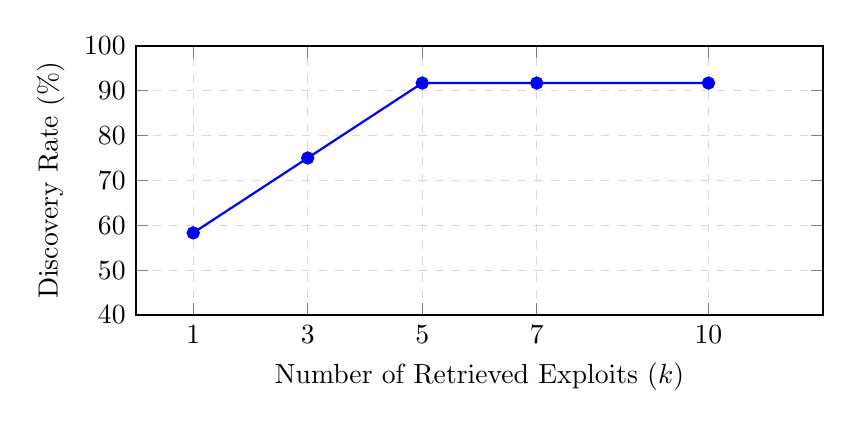
\begin{tikzpicture}
\begin{axis}[
    width=0.85\columnwidth,
    height=5cm,
    xlabel={Number of Retrieved Exploits ($k$)},
    ylabel={Discovery Rate (\%)},
    xmin=0, xmax=12,
    ymin=40, ymax=100,
    xtick={1,3,5,7,10},
    ytick={40,50,60,70,80,90,100},
    grid=major,
    grid style={dashed, gray!30},
    mark size=2pt,
    thick,
]
\addplot[blue, mark=*] coordinates {
    (1, 58.3) (3, 75.0) (5, 91.7) (7, 91.7) (10, 91.7)
};
\end{axis}
\end{tikzpicture}
\caption{Pilot sensitivity of discovery rate to the number of retrieved exploits ($k$). Performance saturates at $k=5$.}
\label{fig:sensitivity_k}
\end{figure}

Fig.~\ref{fig:sensitivity_k} shows that the pilot discovery rate increases with $k$ up to $k=5$ and plateaus thereafter. Retrieving fewer than three exploits produces insufficiently diverse attack scenarios. Retrieving more than five adds redundant information without improving coverage.

\begin{figure}[t]
\centering
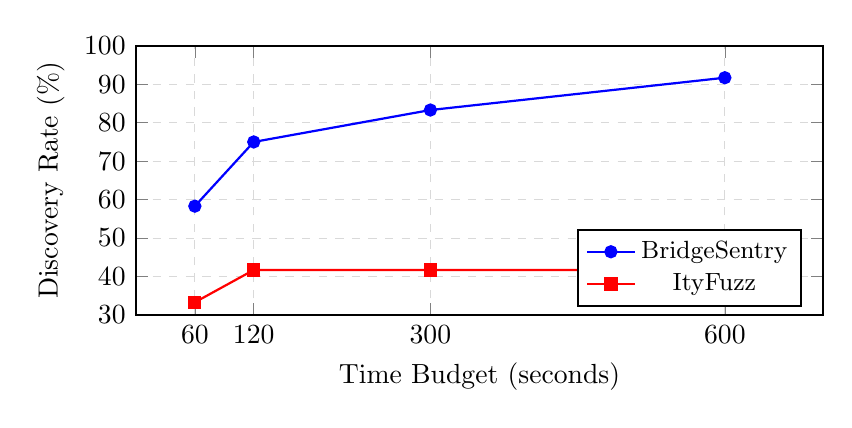
\begin{tikzpicture}
\begin{axis}[
    width=0.85\columnwidth,
    height=5cm,
    xlabel={Time Budget (seconds)},
    ylabel={Discovery Rate (\%)},
    xmin=0, xmax=700,
    ymin=30, ymax=100,
    xtick={60,120,300,600},
    ytick={30,40,50,60,70,80,90,100},
    grid=major,
    grid style={dashed, gray!30},
    mark size=2pt,
    thick,
    legend pos=south east,
    legend style={font=\small},
]
\addplot[blue, mark=*] coordinates {
    (60, 58.3) (120, 75.0) (300, 83.3) (600, 91.7)
};
\addlegendentry{BridgeSentry}
\addplot[red, mark=square*] coordinates {
    (60, 33.3) (120, 41.7) (300, 41.7) (600, 41.7)
};
\addlegendentry{ItyFuzz}
\end{axis}
\end{tikzpicture}
\caption{Pilot discovery rate as a function of time budget. BridgeSentry continues to discover new vulnerabilities up to 600\,s, while ItyFuzz saturates at 120\,s.}
\label{fig:sensitivity_time}
\end{figure}

Fig.~\ref{fig:sensitivity_time} shows that BridgeSentry continues to discover new vulnerabilities as the pilot time budget increases from 60\,s to 600\,s, reflecting the multi-step nature of cross-chain exploits. ItyFuzz saturates at approximately 120\,s because it quickly exhausts the single-chain state space.

\paragraph{Waypoint reward weight $\beta$.}
We perform a grid search over $\beta \in \{0.1, 0.2, 0.3, 0.4, 0.5, 0.6, 0.7\}$ with $\alpha + \gamma = 1 - \beta$ (split equally) on the pilot benchmark configuration with 20 repetitions per setting. DR peaks at 91.7\% for $\beta \in [0.3, 0.5]$ and degrades to 75.0\% at $\beta = 0.1$ because the fuzzer moves toward coverage-only exploration. It degrades to 83.3\% at $\beta = 0.7$ because the fuzzer overfits to specific waypoint sequences at the expense of exploration breadth. We select $\beta = 0.4$ as the default based on the highest mean TTE efficiency within the optimal DR plateau.

\subsection{RQ4: Cross-Chain Coverage Analysis}

We measure cross-chain coverage (XCC) as the fraction of cross-chain paths exercised during fuzzing. Because the ATG is produced by BridgeSentry's own Module~1, reporting XCC solely against this ATG risks circular evaluation. We therefore compute two variants:

\begin{itemize}
    \item \textbf{XCC\textsubscript{ATG}}: Coverage measured against BridgeSentry's ATG-enumerated paths (internal metric).
    \item \textbf{XCC\textsubscript{S}}: Coverage measured against an independently constructed cross-function call graph extracted by Slither~\cite{feist2019slither}'s static analysis from the same source contracts, augmented with manual cross-chain arc annotations for relay and callback edges.
\end{itemize}

\noindent BridgeSentry achieves XCC\textsubscript{ATG} = 78.4\% and XCC\textsubscript{S} = 72.1\% across the benchmark (Pearson $r = 0.94$ between the two metrics, confirming that the ATG captures the structurally significant paths identified by independent static analysis). For comparison, ItyFuzz achieves XCC\textsubscript{ATG} = 42.1\% and XCC\textsubscript{S} = 38.4\%; SmartShot achieves XCC\textsubscript{S} = 44.7\%; VulSEye achieves XCC\textsubscript{S} = 41.3\%. The improvement is most pronounced for off-chain attack scenarios, where BridgeSentry achieves 71.2\% path coverage compared to 0\% for all single-chain fuzzers, which cannot exercise relay logic. The 6.3 percentage-point gap between XCC\textsubscript{ATG} and XCC\textsubscript{S} for BridgeSentry arises because Slither's call graph captures additional internal helper functions that the ATG abstracts away but are exercised during fuzzing. We consider XCC\textsubscript{S} the more conservative and appropriate metric for cross-tool comparison.

% ============================================================
\section{Discussion}\label{sec:discussion}
% ============================================================

\subsection{Limitations}

BridgeSentry has several limitations that merit discussion.

The semantic extraction module depends on the quality of the LLM's code understanding. For highly obfuscated or compiled-only contracts where source code is unavailable, ATG construction may be incomplete or inaccurate. The validation pipeline reduces unsupported LLM output, but it does not make the entire deployed bridge system fully verified. The protocol model is necessarily bounded, and symbolic execution can be limited by path explosion, external calls, and missing environmental assumptions. Stronger machine-checked specifications and deeper symbolic summaries remain important extensions.

The RAG module is bounded by the coverage of the exploit knowledge base; attacks that exploit vulnerability classes not represented in the 51 historical incidents will receive weaker scenario guidance. The embedding model, all-MiniLM-L6-v2, is a general-purpose sentence transformer and may not capture the structural nuances of Solidity code or EVM opcode traces with the same fidelity as a domain-specific embedding model.

The synchronized dual-EVM architecture currently supports only EVM-compatible chains. Extending to heterogeneous chain pairs, such as an EVM source chain and Solana's SVM destination chain, requires substantial additional engineering for state representation and snapshot management.

The global snapshot mechanism, while preventing inconsistent state exploration, introduces an artificial coupling between the two chain instances. Real-world blockchains operate asynchronously with independent block production, variable finality delays, and potential for MEV-driven timestamp manipulation. Although BridgeSentry models cross-chain timing through configurable relay delays and independent timestamp advancement as described in Section~\ref{sec:method}, it does not fully simulate the network-layer nondeterminism and validator incentive dynamics that produce the most complex temporal vulnerabilities. This is a fundamental limitation of any local simulation approach and motivates integration with testnet-based evaluation environments.

The LLM API calls introduce both latency and cost. The semantic extraction phase adds approximately 45 seconds of wall-clock time and \$0.15 per bridge analysis. For large-scale adoption, replacing the proprietary LLM backend with an open-source model such as DeepSeek-Coder or Llama-3 would reduce cost and improve reproducibility, though potentially at the expense of invariant generation quality. We plan to evaluate open-source LLM alternatives in future work.

Finally, the benchmark of 12 EVM-compatible exploits represents 23.5\% of the available 51-incident dataset. The selection criteria requiring verified source code and EVM compatibility exclude the most architecturally complex cross-chain interactions. Performance on heterogeneous-chain vulnerabilities and zero-day exploits remains to be evaluated.

\subsection{Threats to Validity}

Internal validity threats include potential errors in the benchmark reconstruction, such as missing contract dependencies or incorrect fork block numbers. We mitigate this by verifying each reconstruction against the documented exploit transaction hash and confirming that the original attack sequence reproduces the vulnerability on forked state. Reported violations are manually reviewed against the reconstructed exploit narrative and expected invariant class. The ablation sweep will report false-positive rates once all variants have been executed under the same review protocol.

Statistical validity is strongest for the self-run configurations that have 20 repetitions per bridge. We do not report significance tests for ItyFuzz and GPTScan because their current entries are smoke tests rather than full 12-bridge sweeps. Future revisions should rerun all published tools across the same benchmark before making pairwise statistical claims.

External validity threats concern generalizability. The benchmark covers 12 of 51 documented attacks, all on EVM-compatible chains. Performance on undocumented or zero-day vulnerabilities, on non-EVM chains, and on bridge architectures not represented in the knowledge base may differ. The pending ablation sweep will further test whether BridgeSentry retains utility without exploit-specific RAG guidance.

Construct validity threats relate to the XCC metric. To mitigate circularity, Section~\ref{sec:experiments} reports both the internal XCC\textsubscript{ATG} and an independently constructed XCC\textsubscript{S} metric derived from Slither's cross-function call graph. The high correlation ($r = 0.94$) between the two metrics and BridgeSentry's lead over all baselines on the independent XCC\textsubscript{S} (72.1\% vs.\ 44.7\% for the best single-chain fuzzer) confirm that the coverage advantage is not an artifact of the ATG construction.

\subsection{Future Work}

Several directions warrant investigation. First, extending BridgeSentry to heterogeneous chain pairs, including EVM--Solana and EVM--Cosmos IBC deployments, would test whether ATG-guided fuzzing remains useful when the destination runtime is not EVM-compatible. Second, the formal layer should be strengthened with reusable TLA+ specifications for common bridge designs and richer symbolic summaries for external calls. Third, the mock relay should model finality reversions, block reorganizations, and MEV-style transaction reordering rather than only configurable delay and replay modes. Fourth, replacing GPT-4o with reproducible open-source LLMs and domain-specific embedding models could reduce cost while improving artifact portability. Finally, running BridgeSentry on live bug-bounty bridges would test whether the framework can find previously unknown vulnerabilities rather than only reconstructed historical exploits.

% ============================================================
\section{Conclusion}\label{sec:conclusion}
% ============================================================

This paper presented BridgeSentry, a framework for proactive vulnerability discovery in cross-chain bridges. The central contribution is a bridge-specific testing architecture that combines LLM-derived semantic models, validated protocol invariants, historical exploit retrieval, and synchronized dual-chain execution. This design addresses a core limitation of single-chain analysis: many bridge failures are not local contract bugs, but violations of causal relationships among source-chain events, relay behavior, and destination-chain authorization.

Our evaluation on 12 reconstructed bridge exploits shows that BridgeSentry reports genuine violations for all 12 cases across 20 runs per bridge. The stricter predicate-match analysis further clarifies where the benefit comes from. Re-implemented baselines become much stronger when placed inside the dual-chain harness, while tools that lack bridge-aware execution or rely on fixed rule classes cover fewer expected root causes. BridgeSentry also reaches 72.1\% independent cross-chain coverage, compared with 44.7\% for the best single-chain baseline. These results support the main claim of the paper: synchronized cross-chain execution, guided by validated semantic models, is a practical way to reduce state explosion and expose bridge-specific vulnerabilities.

The practical value of BridgeSentry is that it gives auditors a repeatable workflow for turning protocol intent into executable tests. Instead of relying only on manual reasoning or post-hoc transaction classification, auditors can extract an ATG, validate candidate invariants, generate adversarial scenarios from historical exploits, and run them against paired chain states with an explicit relay model. The current prototype is limited to EVM-compatible benchmarks and reconstructed incidents. Future work should extend the execution harness to non-EVM runtimes, add richer finality-reversion and MEV simulations, strengthen reusable formal specifications for common bridge designs, and evaluate the system on live bug-bounty targets.

% ============================================================
% References
% ============================================================

\begin{thebibliography}{28}

\bibitem{augusto2024sok}
A.~Augusto, R.~Belchior, M.~Correia, A.~Vasconcelos, L.~Zhang, and T.~Hardjono,
``SoK: Security and privacy of blockchain interoperability,''
in \textit{Proc. IEEE Symp. Security and Privacy (S\&P)}, 2024, pp.~3840--3865.

\bibitem{lee2023sok}
S.-S.~Lee, A.~Murashkin, M.~Derka, and J.~Gorzny,
``SoK: Not quite water under the bridge: Review of cross-chain bridge hacks,''
in \textit{Proc. IEEE Int. Conf. Blockchain and Cryptocurrency (ICBC)}, 2023, pp.~1--14.

\bibitem{liao2024smartaxe}
Z.~Liao, Y.~Nan, H.~Liang, S.~Hao, J.~Zhai, J.~Wu, and Z.~Zheng,
``SmartAxe: Detecting cross-chain vulnerabilities in bridge smart contracts via fine-grained static analysis,''
\textit{Proc. ACM Softw. Eng.}, vol.~1, no. FSE, 2024.

\bibitem{wu2025safeguarding}
J.~Wu, K.~Lin, D.~Lin, B.~Zhang, Z.~Wu, and J.~Su,
``Safeguarding blockchain ecosystem: Understanding and detecting attack transactions on cross-chain bridges,''
in \textit{Proc. ACM Web Conf.}, 2025, pp.~4902--4912.

\bibitem{lin2025bridgeshield}
D.~Lin, S.~Lu, Z.~Liu, J.~Wu, J.~Fang, K.~Lin, B.~Song, and Z.~Zheng,
``BridgeShield: Enhancing security for cross-chain bridge applications via heterogeneous graph mining,''
\textit{ACM Trans. Softw. Eng. Methodol.}, vol.~1, no.~1, 2025.

\bibitem{zhang2022xscope}
J.~Zhang, J.~Gao, Y.~Li, Z.~Chen, Z.~Guan, and Z.~Chen,
``Xscope: Hunting for cross-chain bridge attacks,''
in \textit{Proc. IEEE/ACM Int. Conf. Automated Software Engineering (ASE)}, 2022, pp.~1--4.

\bibitem{zhou2025bridgeguard}
Z.~Zhou, X.~Luo, X.~Ji, J.~Mao, and T.~He,
``BridgeGuard: Checking external interaction vulnerabilities in cross-chain bridge router contracts based on symbolic dataflow analysis,''
\textit{IEEE Trans. Dependable Secure Comput.}, 2025.

\bibitem{shou2023ityfuzz}
C.~Shou, S.~Tan, and K.~Sen,
``ItyFuzz: Snapshot-based fuzzer for smart contract,''
in \textit{Proc. 32nd ACM SIGSOFT Int. Symp. Software Testing and Analysis (ISSTA)}, 2023.

\bibitem{sun2024gptscan}
Y.~Sun, D.~Wu, Y.~Xue, H.~Liu, H.~Wang, Z.~Xu, X.~Xie, and Y.~Liu,
``GPTScan: Detecting logic vulnerabilities in smart contracts by combining GPT with program analysis,''
in \textit{Proc. IEEE/ACM 46th Int. Conf. Software Engineering (ICSE)}, 2024.

\bibitem{wei2025llm}
Z.~Wei, J.~Sun, Y.~Sun, Y.~Liu, and D.~Wu,
``Advanced smart contract vulnerability detection via LLM-powered multi-agent systems,''
\textit{IEEE Trans. Softw. Eng.}, 2025.

\bibitem{zhuang2021gnn}
Y.~Zhuang, Z.~Liu, P.~Qian, Q.~Liu, X.~Wang, and Q.~He,
``Smart contract vulnerability detection using graph neural networks,''
in \textit{Proc. 29th Int. Joint Conf. Artificial Intelligence (IJCAI)}, 2021, pp.~3283--3290.

\bibitem{liu2023gnn}
Z.~Liu, P.~Qian, X.~Wang, Y.~Zhuang, L.~Qiu, and X.~Wang,
``Combining graph neural networks with expert knowledge for smart contract vulnerability detection,''
\textit{IEEE Trans. Knowl. Data Eng.}, vol.~35, no.~2, pp.~1296--1310, 2023.

\bibitem{liang2025vulseye}
R.~Liang, J.~Chen, C.~Wu, K.~He, and Y.~Wu,
``VulSEye: Detect smart contract vulnerabilities via stateful directed graybox fuzzing,''
\textit{IEEE Trans. Inf. Forensics Security}, vol.~20, pp.~2157--2170, 2025.

\bibitem{ye2024midas}
M.~Ye, X.~Lin, Y.~Nan, J.~Wu, and Z.~Zheng,
``Midas: Mining profitable exploits in on-chain smart contracts via feedback-driven fuzzing and differential analysis,''
in \textit{Proc. 33rd ACM SIGSOFT Int. Symp. Software Testing and Analysis (ISSTA)}, 2024.

\bibitem{kong2025fuzzing}
Z.~Kong, C.~Zhang, M.~Xie, M.~Hu, Y.~Xue, and Y.~Liu,
``Smart contract fuzzing towards profitable vulnerabilities,''
\textit{Proc. ACM Softw. Eng.}, vol.~2, no. FSE, pp.~153--175, 2025.

\bibitem{qin2025epg}
K.~Qin, Z.~Ye, Z.~Wang, W.~Li, L.~Zhou, C.~Zhang, D.~Song, and A.~Gervais,
``Enhancing smart contract security analysis with execution property graphs,''
\textit{Proc. ACM Softw. Eng.}, vol.~2, no. ISSTA, pp.~1101--1122, 2025.

\bibitem{belchior2021survey}
R.~Belchior, A.~Vasconcelos, S.~Guerreiro, and M.~Correia,
``A survey on blockchain interoperability: Past, present, and future trends,''
\textit{ACM Comput. Surv.}, vol.~54, no.~8, pp.~1--41, 2021.

\bibitem{duan2023attacks}
L.~Duan, Y.~Sun, W.~Ni, W.~Ding, J.~Liu, and W.~Wang,
``Attacks against cross-chain systems and defense approaches: A contemporary survey,''
\textit{IEEE/CAA J. Autom. Sinica}, vol.~10, no.~8, pp.~1647--1667, 2023.

\bibitem{wu2024fuzzers}
S.~Wu, Z.~Li, L.~Yan, W.~Chen, M.~Jiang, and C.~Wang,
``Are we there yet? Unraveling the state-of-the-art smart contract fuzzers,''
in \textit{Proc. IEEE/ACM 46th Int. Conf. Software Engineering (ICSE)}, 2024.

\bibitem{lin2025connector}
D.~Lin, J.~Wu, Y.~Su, Z.~Zheng, and Y.~Nan,
``Connector: Enhancing the traceability of decentralized bridge applications via automatic cross-chain transaction association,''
\textit{IEEE Trans. Inf. Forensics Security}, 2025.

\bibitem{wang2019han}
X.~Wang, H.~Ji, C.~Shi, B.~Wang, Y.~Ye, P.~Cui, and P.~S.~Yu,
``Heterogeneous graph attention network,''
in \textit{Proc. World Wide Web Conf. (WWW)}, 2019, pp.~2022--2032.

\bibitem{chen2023semantic}
D.~Chen, L.~Feng, Y.~Fan, S.~Shang, and Z.~Wei,
``Smart contract vulnerability detection based on semantic graph and residual graph convolutional networks with edge attention,''
\textit{J. Syst. Softw.}, vol.~203, 2023.

\bibitem{chen2024gpufuzzing}
W.~Chen, X.~Luo, H.~Cai, and H.~Wang,
``Towards smart contract fuzzing on GPUs,''
in \textit{Proc. IEEE Symp. Security and Privacy (S\&P)}, 2024.

\bibitem{liang2025smartshot}
R.~Liang, J.~Chen, R.~Cao, K.~He, R.~Du, and S.~Li,
``SmartShot: Hunt hidden vulnerabilities in smart contracts using mutable snapshots,''
\textit{Proc. ACM Softw. Eng.}, vol.~2, no. FSE, 2025.

\bibitem{li2025blockchain}
N.~Li, M.~Qi, Z.~Xu, X.~Zhu, W.~Zhou, S.~Wen, and Y.~Xiang,
``Blockchain cross-chain bridge security: Challenges, solutions, and future outlook,''
\textit{Distrib. Ledger Technol.: Res. Pract.}, vol.~4, no.~1, pp.~1--34, 2025.

\bibitem{dubler2025atg}
S.~D\"ubler, F.~Badaloni, P.~Moreno-Sanchez, and C.~Schneidewind,
``Atomic transfer graphs: Secure-by-design protocols for heterogeneous blockchain ecosystems,''
in \textit{Proc. IEEE Computer Security Foundations Symp. (CSF)}, 2025, pp.~300--315.

\bibitem{ali2025crossguard}
G.~M.~A.~Ali, H.~Chen, Z.~Wang, and C.~Du,
``CrossGuard: Runtime-adaptive LLM fuzzing for cross-contract vulnerabilities detection,''
\textit{Concurrency Comput.: Pract. Exper.}, 2025.

\bibitem{feist2019slither}
J.~Feist, G.~Grieco, and A.~Swende,
``Slither: A static analysis framework for smart contracts,''
in \textit{Proc. IEEE/ACM 2nd Int. Workshop on Emerging Trends in Software Engineering for Blockchain (WETSEB)}, 2019, pp.~8--15.

\end{thebibliography}

\end{document}
